% !TeX encoding=utf8
% !TeX spellcheck=de-DE
% !TeX root=../UID_Project_Documentation.tex

\section{Motivation}

\subsection{Einordnung und Problemstellung}

Das von uns erdachte Produkt beschäftigt sich mit Problemen, die beim Anbieten und Konsumieren von ehemaligen Print-Inhalten im digitalen Zeitalter entstehen und die wir als von den bisherigen Angeboten ungelöst sehen.

Mit dem Einzug von digitalen Gerätschaften und dem Internet in die Haushalte und den Alltag eines großen Teils der Weltbevölkerung ist die Nachfrage nach digitalen Inhalten jedweder Form stark und stetig gestiegen. Auch der Journalismus ist von dieser Entwicklung nicht verschont geblieben und es wird seitdem versucht sich entsprechend anzupassen. Zum Beispiel war bereits am 25. Oktober 1994 mit \enquote{Spiegel Online} eine von Deutschlands bekanntesten Quellen für Journalismus über das Netz erreichbar. Heute vertreibt praktisch jede professionelle Publikation ihre Inhalte zumindest teilweise über einen Webauftritt und muss sich dabei nicht nur gegenüber der traditionellen Konkurrenz sondern auch einer schier unzählige Masse an privaten und halb-professionellen \enquote{Bloggern} behaupten.

Diese neuen Gefilde zeigen einige Dynamiken und Aspekte auf, die sich von denen der traditionellen Vertriebswelt für Journalismus stark unterscheiden. Der moderne Nutzer ist es gewohnt alle Inhalte die er wünscht direkt abrufbar zu haben. Es ist normal verschiedenste Quellen zu konsumieren, um entweder ihre Inhalte zu einem bestimmten Thema zu vergleichen oder vielmehr sie den Schwerpunkten ihrer Kompetenz gerecht zu nutzen um sich so eine persönliche, optimierte Konsumlandschaft zu kreieren.

Durch dieses Konsumverhalten zusammen mit der stärkeren Konkurrenz an diesem transparenteren Markt, sowie den technischen Limitationen des Mediums, stellt sich das Monetarisieren von digitalen Inhalten als eine nicht zu unterschätzende Herausforderung dar.

Das einzige Geschäftsmodell, welches sich bisher wirklich durchgesetzt hat ist die Monetarisierung durch das Schalten von Werbeanzeigen. Dieses bringt allerdings einige Problemen mit sich. Durch dieses Modell wird die Wirtschaftlichkeit eines Inhalts ausschließlich durch die von ihm generierte Anzahl an Aufrufen bestimmt. Dadurch wird der Konsument der Inhalte vom Kunden der Publikationen zu deren Produkt, welches diese an die Werbeschaltenden verkaufen. Dadurch rückt der eigentliche Kunde aus dem Fokus und die Tatsache dass Werbeanzeigen generell als störend empfunden werden, wird hingenommen. Tendenziell belohnt das Modell Quantität mehr als Qualität und dadurch kurze, Aufmerksamkeit heischende Beiträge mehr als fundierte, differenzierte Berichterstattung. Vor allem aber, rechnet es sich erst ab einer hohen absoluten Zahl von Aufrufen und ist auch dann oft nicht ausreichend. Zum Beispiel erwirtschaftet die international erfolgreiche, britische Publikation \enquote{The Guardian} seit Jahren nur Verluste und muss sich durch andere Publikationen querfinanzieren.

Hieraus ergibt sich eine Situation, welche sowohl für den Konsumenten als auch für den Produzenten der Inhalte unvorteilhaft ist und wir wurden das Gefühl nicht los, dass es doch eine bessere Lösung geben muss.

\subsection{Konzept}

Wir wollten eine Lösung gestalten, die dem Nutzer all die Freiheit und Flexibilität gibt, die er von einem modernen Dienst gewohnt ist und erwartet, jedoch auch für die Anbieter von Inhalten eine effektive und faire Form der Monetarisierung darstellt. Das ganze sollte abgerundet werden durch eine intuitive und leichte Nutzererfahrung, welche die Hürden für das Verwenden unseres Dienstes und das Konsumieren von monetarisierten Inhalten durch ihn so weit wie möglich senkt.

Hierfür haben wir eine Nachrichten App entworfen, welche Inhalte von Verschiedensten Quellen auf einer möglichst granularen Ebene bereitstellt. Das bedeutet, dass man grundsätzlich für jeden Inhalt einzeln bezahlen kann oder aber auch bestimmte Sammlungen von Inhalten abonnieren kann. In der Praxis könnte man so das \enquote{Sport}-Segment von Zeitung A abonnieren, sowie alle Artikel die von Autor P geschrieben werden, die Komplette Zeitung B, als auch vereinzelte Artikel von den Zeitschriften C, D und E. Wir versuchen so die Vorteile von On-Demand- sowie Flatrate-Modellen zu nutzen. Ein Nutzer kann sich die von ihr gekauften oder abonnierten Inhalte dann in sogenannten Feeds zusammenstellen und so ihren Konsum stark personalisieren.

Bisherige Produkte, welche ehemals Print-Inhalte digital anbieten, haben zwar einige der beschriebenen Probleme gelöst indem sie ihren Kunden einen Single-Point-of-Access (SPA) für die Inhalte mehrerer Publikationen sowie die damit zusammenhängenden Transaktionen bieten. Allerdings, haben sie nicht den revolutionären Schritt getan die Struktur der Angebotenen Inhalte aufzubrechen und den Nutzern somit umfangreiche Personalisierungsmöglichkeiten beim Konsum als auch Flexibilität beim Kauf zu ermöglichen. Deswegen sind wir überzeugt, dass sich unser Produkt in dem Oligopol der digitalen Nachrichten-Plattformen gegen die Konkurrenz behaupten kann.

Während wir in dieser Ausarbeitung nur die Umsetzung unseres Konzepts als Smartphone-App ausführen, so wären in einem realen Szenario jedoch auch eine Webapp, sowie angepasste Anwendungen für alle anderen gängigen Systeme Teil der Umsetzung. Hierbei würde man sich um ein möglichst eingängiges Design bemühen um Nutzern ein möglichst uniformes Erlebnis zu ermöglichen, sowie von Vertrautheit und Wiedererkennungswert zu profitieren.

\clearpage

\section{Observation}

\subsection{Marktanalyse}

Das Produkt befindet sich im Marktsegment der Online Nachrichten. Dieses Marktsegment lässt sich noch weiter Einteilen: Nachrichtenseiten der Anbieter (z.~B. Fernsehsender, Printmedien Anbieter), Soziale Netzwerke und Nachrichtenseiten, die nicht zu klassischen Medienhäusern gehören. D.~h., dass bei diesen Nachrichtenseiten, Nachrichten von klassischen Medienhäusern genutzt werden und zentralisiert auf diesen Seiten angezeigt werden. Laut einer Bitkom Studie hat diese Art der Online Nachrichten den geringsten Anteil zu den anderen Sub Segmenten von Online Nachrichten mit 7\% Marktanteil.\footnote{
  \begin{sloppypar}
    \url{https://de.statista.com/statistik/daten/studie/532213/umfrage/nutzung-von-nachrichten-nach-quellen-im-internet-in-deutschland}
  \end{sloppypar}
}

Bei Betrachtung der monatlichen Ausgaben für Online Nachrichten gibt es folgende Verteilung\footnote{
  \begin{sloppypar}
    \url{https://de.statista.com/statistik/daten/studie/71492/umfrage/paid-content-ausgaben-fuer-online-news-in-deutschland-in-2009}
  \end{sloppypar}
}

\begin{itemize}
  \item 0€ - 75\%
  \item 1€-5€ - 10\%
  \item 6€-10€ - 6\%
  \item Über 10€ - 9\%
\end{itemize}

Im Vergleich mit anderen digitalen Inhalten, wird für Online Nachrichten am zweitwenigsten ausgegeben (15,6\%) danach folgt sonstiges (1,1\%), welches mehrere digitale Inhalte zusammenfasst. Den größten Anteil für bezahlte digitale Inhalte haben Musik und Filme und Serien.\footnote{
  \begin{sloppypar}
    \url{https://de.statista.com/statistik/daten/studie/514812/umfrage/paid-content-nutzung-in-deutschland-nach-segmenten}
  \end{sloppypar}
}

Für die Nutzung von Online Nachrichten ergibt sich für die Nutzung nach Endgerät, dass die meisten Nutzer Smartphones benutzen. Danach folgen Notebooks, Desktops und Tablets.\footnote{
  \begin{sloppypar}
    \url{https://de.statista.com/statistik/daten/studie/511566/umfrage/lesen-von-online-nachrichten-nach-endgeraeten-in-deutschland}
  \end{sloppypar}
}

Bei den Nutzungs Gelegenheiten wird statistisch am häufigsten \enquote{Zuhause in der Freizeit} das Angebot von Online Nachrichten Anbietern genutzt. Danach kommen \enquote{Weg zur Arbeit}, \enquote{Unterwegs in der Freizeit}, \enquote{Während der Arbeit}, \enquote{In der Mittagspause}, \enquote{Auf dem Weg nach Hause}, \enquote{Am Frühstückstisch} und zuletzt \enquote{Abends im Bett}.

Die größten Mitbewerber des Produkts sind \enquote{upday} von Samsung und Axel Springer oder \enquote{Play Kiosk} aka \enquote{Play Newsstand} von Google.

\enquote{upday} ist nur als App auf Samsung Geräten (Android und IoT Geräte) verfügbar. Sie nutzt Machine Learning, um dem Nutzer die optimale Mischung an Nachrichten für den jeweiligen Nutzer zusammenzustellen. Die Nachrichten werden außerdem Zusammengefasst angezeigt. Die App verwendet zu den Nachrichten passende Werbe-Einblendungen.\footnote{
  \begin{sloppypar}
    \url{https://www.welt.de/print/die_welt/wirtschaft/article145911513/Axel-Springer-und-Samsung-starten-Zusammenarbeit.html}
  \end{sloppypar}
}

\enquote{Play Kiosk} ist als App (Android und iOS) und Web-App verfügbar. Es werden Nachrichten geordnet nach den Anbieter oder Themengebiet angezeigt. Es gibt sowohl ein kostenloses als auch ein kostenpflichtiges Angebot. Bei dem kostenpflichtigen Angebot wird ein monatlicher Zugang (für die Nachrichten eines Anbieters) für einen festen Preis Angeboten. Es gibt die Möglichkeit das Bezahlangebot 14 Tage lang kostenlos zu testen. Es gibt nicht die Möglichkeit einzelne Teilbereiche des kostenpflichtigen Angebots freizuschalten, oder mit einer monatlichen Gebühr alle kostenpflichtigen Inhalte freizuschalten. Die kostenlosen Inhalte werden mit Werbung angezeigt.

Es gibt noch weitere Online-Nachrichten Anbieter, wie \enquote{Flipboard}, \enquote{News360}, \enquote{Bundle News}, \enquote{Inoreader}, \enquote{Feedly}. Diese Produkte haben ein ähnliches Angebot, wie die näher vorgestellten Produkte. Die in diesem Absatz genannten Produkte haben keine kostenpflichtigen Inhalte, sondern zeigen ihre kostenlosen Inhalte mit Werbung.

\textbf{Zusammenfassung:}

\begin{itemize}
  \item Hoher Wettbewerb und etablierte Produkte für Online-Nachrichten-Anbieter
  \item Geringe Zahlungsbereitschaft der Nutzer
  \item Kostenpflichtige Inhalte nur von Google und den Angeboten der Medienhäuser selbst
  \item Produkte in diesem Sektor müssen auf allen gängigen Plattformen verfügbar sein. Besonders auf Mobilgeräten
\end{itemize}

\subsection{Personas}

Personas stellen eine Menge von potentiellen Nutzern der App dar. Mit den verschiedenen definierten Nutzerverhalten und Eigenschaften können wir uns als Projektteam besser verschiedene Lösungen für die Bedürfnisse der einzelnen definierten Personas überlegen und umsetzen. Mit den Bild im Kopf können wir uns an den Wünschen und Frustrations der einzelnen Personen orientieren. Bei den Personas haben wir auf unterschiedliche Charaktere gesetzt. Unser Projekt spricht eine breite Zielgruppe an. Egal ob jung oder alt, Mann oder Frau, technikaffin oder nicht, unsere App muss alle dieser Nutzer ansprechen. Innerhalb des Teams haben wir zwei zweier Teams gebildet die jeweils eine eigene Persona erstellt haben. Wir hatten nur die Bedingung, dass die Personas sich grundlegend unterscheiden müssen und sich nicht zu stark überschneiden dürfen. Um einen Unique Selling Point für unsere App zu schaffen, gehen die Personas auf nicht genutztes Potenzial des Marktes ein, die in der Marktanalyse aufgekommen sind. Mit dieser herangehensweise versuchen wir die Observation Phase des UCD Prozess konsistent zu gestalten, um eindeutige Anforderungen für die darauffolgenden Phasen abzuleiten.

\clearpage

\subsubsection{Proto Persona}

\begin{figure}[h]
  \centering
  \includegraphics[width=\textwidth-2cm]{protopersona}
  \caption{Unsere Proto Persona}
  \label{protopersona}
\end{figure}

\subsubsection{Finale Personas}

\clearpage

\section{Ideation}

\subsubsection{Sketches}

Bei den Sketches haben wir uns grundlegend überlegt, wie die App die Anforderungen der potenziellen Nutzer, die durch unsere Personas repräsentiert werden, gelöst werden könnten. Ein wichtiger Punkt dabei ist es den Spagat zwischen der unterschiedlichen Technikaffinität der Personas zu bedienen. Beispielsweise sollen so wenig wie möglich Kognitionsfehler bei den Nutzern entstehen und auch bei erfahrenen Nutzern so wenig wie möglich Routinefehler. Die Sketches stellen Lösungen für die Probleme der Personas dar, die in die Prototyping Phase des UCD Prozess einfließen, um den Prototypen zu gestalten. Eine weitere Herausforderung einer News-App ist, dass sehr viel Inhalt auf übersichtliche Art und Weise auf sehr begrenztem Platz untergebracht werden muss.

\begin{figure}[h]
  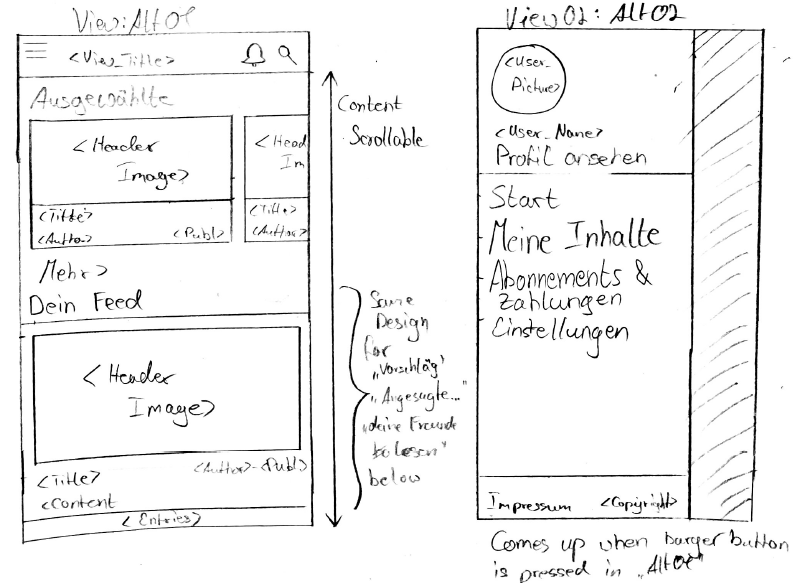
\includegraphics[width=\textwidth]{sketches 01}
  \caption{Sketch 1}
  \label{}
\end{figure}



\section{Prototyping}
\section{Evaluation}
\section{Iteration}
